\documentclass{aion}

% ------------------------------------------------------------
% Metadata for this paper
% ------------------------------------------------------------
\renewcommand{\papertitle}{WARP Graphs: Ethics of Deterministic Replay \& Provenance Sovereignty}
\renewcommand{\papernumber}{Paper V}
\renewcommand{\paperdate}{December 2025}

\renewcommand{\paperauthor}{James Ross}
\renewcommand{\paperaffiliation}{Independent Researcher}
\renewcommand{\paperorcid}{0009-0006-0025-7801}

% ------------------------------------------------------------
% Extra packages needed by this paper
% ------------------------------------------------------------
\usepackage{float}
\usepackage{tikz}
\usetikzlibrary{arrows.meta,positioning,decorations.pathreplacing}

\input{macros}
\newcommand{\AIONDiagramHolography}{
\begin{tikzpicture}[
    state/.style={circle, draw, fill=gray!20, minimum size=8mm, inner sep=0pt},
    boundary/.style={draw, rounded corners, thick, dashed, inner sep=6pt}
  ]
  \node[state] (u0) at (0,0) {$U_0$};
  \node[state] (u1) at (2,0) {$U_1$};
  \node[state] (u2) at (4,0) {$U_2$};
  \node[state] (un) at (6,0) {$U_n$};

  \draw[->, thick] (u0) -- (u1) node[midway, above] {\scriptsize $\mu_0$};
  \draw[->, thick] (u1) -- (u2) node[midway, above] {\scriptsize $\mu_1$};
  \draw[->, thick] (u2) -- (un) node[midway, above] {\scriptsize $\cdots$};

  \node[boundary, fit=(u0)] (b0) {};
  \node[below=2mm of b0] {\scriptsize $U_0$};

  \node[boundary, fit=(u0) (u1) (u2)] (bp) {};
  \node[below=2mm of bp] {\scriptsize payload $P$};

  \node[boundary, fit=(u0) (bp)] (b) {};
  \node[above=2mm of b] {\scriptsize boundary $(U_0,P)$};

  \draw[->, thick, dashed] (b.east) to[out=0,in=180] (un.west);
\end{tikzpicture}
}

\newcommand{\AIONDiagramWormhole}{
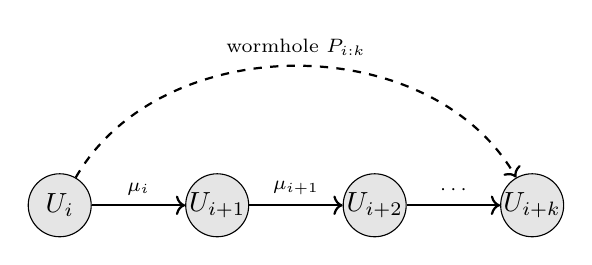
\begin{tikzpicture}[
    state/.style={circle, draw, fill=gray!20, minimum size=8mm, inner sep=0pt},
    wormhole/.style={->, thick, dashed},
    normal/.style={->, thick}
  ]
  \node[state] (u0) at (0,0) {$U_i$};
  \node[state] (u1) at (2,0) {$U_{i+1}$};
  \node[state] (u2) at (4,0) {$U_{i+2}$};
  \node[state] (uk) at (6,0) {$U_{i+k}$};

  \draw[normal] (u0) -- (u1) node[midway, above] {\scriptsize $\mu_i$};
  \draw[normal] (u1) -- (u2) node[midway, above] {\scriptsize $\mu_{i+1}$};
  \draw[normal] (u2) -- (uk) node[midway, above] {\scriptsize $\cdots$};

  \draw[wormhole] (u0) to[out=60,in=120] node[midway, above] {\scriptsize wormhole $P_{i:k}$} (uk);
\end{tikzpicture}
}

\newcommand{\AIONDiagramSlicing}{
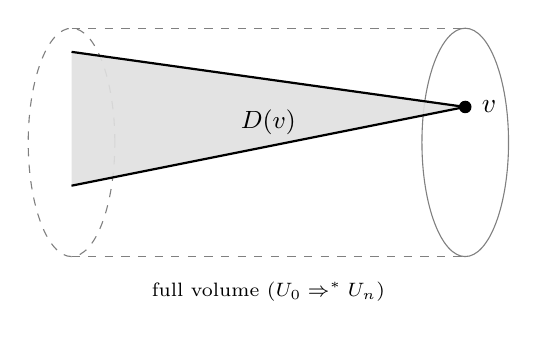
\begin{tikzpicture}
  % Bulk "volume" cylinder
  \draw[gray, dashed] (0,0) ellipse (0.55 and 1.45);
  \draw[gray] (5,0) ellipse (0.55 and 1.45);
  \draw[gray, dashed] (0,1.45) -- (5,1.45);
  \draw[gray, dashed] (0,-1.45) -- (5,-1.45);

  % Backward cone (derivation graph)
  \node[circle, fill=black, inner sep=1.6pt, label=right:$v$] (v) at (5, 0.45) {};
  \fill[black!12, opacity=0.9] (5, 0.45) -- (0, -0.55) -- (0, 1.15) -- cycle;
  \draw[black, thick] (5, 0.45) -- (0, -0.55);
  \draw[black, thick] (5, 0.45) -- (0, 1.15);

  \node at (2.5, 0.25) {\small $D(v)$};
  \node[align=center, font=\scriptsize, below] at (2.5, -1.65) {full volume ($U_0 \Rightarrow^* U_n$)};
\end{tikzpicture}
}

\newcommand{\AIONDiagramForkAndWormhole}{
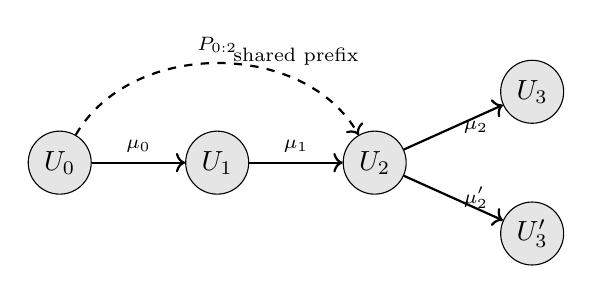
\begin{tikzpicture}[
    state/.style={circle, draw, fill=gray!20, minimum size=8mm, inner sep=0pt},
    normal/.style={->, thick},
    wormhole/.style={->, thick, dashed},
    fork/.style={->, thick}
  ]
  \node[state] (u0) at (0,0) {$U_0$};
  \node[state] (u1) at (2,0) {$U_1$};
  \node[state] (u2) at (4,0) {$U_2$};
  \node[state] (u3) at (6,0.9) {$U_3$};
  \node[state] (u3p) at (6,-0.9) {$U_3'$};

  % Full (uncompressed) prefix
  \draw[normal] (u0) -- (u1) node[midway, above] {\scriptsize $\mu_0$};
  \draw[normal] (u1) -- (u2) node[midway, above] {\scriptsize $\mu_1$};

  % Wormhole compression of the prefix
  \draw[wormhole] (u0) to[out=60,in=120] node[midway, above] {\scriptsize $P_{0:2}$} (u2);

  % Fork at next tick
  \draw[fork] (u2) -- (u3) node[midway, right] {\scriptsize $\mu_2$};
  \draw[fork] (u2) -- (u3p) node[midway, right] {\scriptsize $\mu_2'$};

  \node[font=\scriptsize] at (3,1.35) {shared prefix};
\end{tikzpicture}
}

\newcommand{\AIONDiagramReplayLifecycle}{
\begin{tikzpicture}[
    x=0.55cm, y=0.58cm,
    process/.style={draw, rounded corners=2pt, align=center, minimum height=7mm, text width=16mm, inner sep=1.8pt},
    processwide/.style={process, text width=18mm},
    decision/.style={draw, diamond, aspect=2.0, align=center, inner sep=1pt, text width=12mm},
    flow/.style={->, thick, >=Latex},
    font=\scriptsize
  ]
  % Main vertical path
  \node[process] (n1) at (0.0, 0.0) {1. Replay\\request};
  \node[process] (n2) at (0.0, -2.1) {2. Role\\authority\\validation};
  \node[process] (n3) at (0.0, -4.2) {3. Policy\\constraint check};
  \node[decision] (n4) at (0.0, -6.3) {4.\\Decision};
  \node[process] (n6) at (0.0, -8.4) {6. Execution};
  \node[process] (n7) at (0.0, -10.5) {7. Tamper-evident\\logging};
  \node[process] (n8) at (0.0, -12.6) {8. Review\\trigger};

  % Branch nodes
  \node[process] (n5) at (-4.0, -8.4) {5. Emergency\\override warrant};
  \node[processwide] (n9) at (4.0, -12.6) {9. Dispute /\\arbiter path};
  \node[processwide] (n10) at (8.0, -12.6) {10. Closure +\\evidence bundle};

  % Flows
  \draw[flow] (n1) -- (n2);
  \draw[flow] (n2) -- (n3);
  \draw[flow] (n3) -- (n4);

  \draw[flow] (n4.south) -- node[right] {\tiny approve} (n6.north);
  \draw[flow] (n6) -- (n7);
  \draw[flow] (n7) -- (n8);
  \draw[flow] (n8.east) -- (n9.west);
  \draw[flow] (n9) -- (n10);

  \draw[flow] (n4.south west) to[out=-145, in=90] node[left, pos=0.55] {\tiny emergency} (n5.north);
  \draw[flow] (n5.east) -- (n6.west);
  \draw[flow] (n4.east) to[out=10, in=90] node[above right, pos=0.58] {\tiny deny} (n9.north);
\end{tikzpicture}
}


% ------------------------------------------------------------
% Notation shortcuts (guarded to avoid clashes)
% ------------------------------------------------------------
\ifdefined\WCat\else\newcommand{\WCat}{\mathcal{W}}\fi
\ifdefined\AION\else\newcommand{\AION}{AI$\Omega$N}\fi
\ifdefined\COMPUTER\else\newcommand{\COMPUTER}{C$\Omega$MPUTER}\fi
\ifdefined\sectionbreak\else\newcommand{\sectionbreak}{\clearpage}\fi
\ifdefined\cref\else\newcommand{\cref}{\ref}\fi

% Rewrite / evolution notation (if not already provided by macros.tex)
\ifdefined\Rewrite\else\newcommand{\Rewrite}{\Rightarrow}\fi
\ifdefined\Apply\else\newcommand{\Apply}{\operatorname{Apply}}\fi
\ifdefined\Recon\else\newcommand{\Recon}{\operatorname{Recon}}\fi

% Give hyperref unique anchors for figures to silence duplicate-destination warnings
\makeatletter
\renewcommand{\theHfigure}{\thesection.\arabic{figure}}
\makeatother

\begin{document}

\AIONTitlePage

\cleardoublepage
\thispagestyle{empty}

\begin{center}
{\small
\vspace*{\fill}

\textcopyright~2025 James Ross\\[0.75em]

This work is licensed under the\\
\textbf{Creative Commons Attribution 4.0 International License (CC BY 4.0).}\\[1em]

You are free to:
\begin{itemize}[leftmargin=2em]
  \item \textbf{Share} — copy and redistribute the material in any medium or format
  \item \textbf{Adapt} — remix, transform, and build upon the material for any purpose
\end{itemize}

Under the following terms:
\begin{itemize}[leftmargin=2em]
  \item \textbf{Attribution} — You must give appropriate credit, provide a link to the license,\\
        and indicate if changes were made. You may not imply endorsement by the author.
\end{itemize}

For the full legal code of the license, see:\\[0.25em]
\url{https://creativecommons.org/licenses/by/4.0/}

\vspace*{\fill}
}
\end{center}

\cleardoublepage

\begin{abstract}
When a computer can record and deterministically replay a complete thought process---including hybrid human--machine cognition---that capability is not neutral.
It is access to interior life in executable form.

This paper isolates the ethical consequences of deterministic replay, complete provenance capture, and counterfactual forking in the \WARP{} programme.
We formalise \emph{provenance sovereignty}: an agent's right to control capture, inspection, replay, and branching of its worldline, with special attention to hybrid cognition where human reasoning is partially implemented on \AION{}-style substrates.

Building on The Open Charter v6.1.0~\cite{ross_open_charter_v6_1}, we make the adversarial threat model explicit (replay-as-torture, cognitive extraction, fork-bombing), argue that near-term ``AI debugging'' norms will be inherited by future neurotechnology, and provide conservative operational triggers for the system-mode/mind-mode boundary.
We propose runtime-level requirements---revocable consent, capability-scoped observers, cryptographic sealing, fork rights with creator obligations, and a concrete Charter-warrant protocol for emergency override---and show how they constrain replay tooling and provenance payload formats.
\end{abstract}

\clearpage
\tableofcontents
\clearpage

\section{Introduction}
\label{sec:intro}

The first four papers in the \WARP{} Foundations series develop a technical thesis:
for a wide class of graph-based computations, we can enforce determinism in concurrent rewriting,
and we can make provenance \emph{complete} in the sense that suitably structured boundary data
determines the interior of an execution.

That technical thesis has an immediate ethical shadow.
If a system can replay and inspect every microstep of a computation, then for systems that implement
cognition the provenance stream is not merely a diagnostic artefact; it is (potentially) an interior
life in executable form.
And once we can fork a recorded worldline into counterfactual continuations, a runtime can instantiate
new descendants whose moral status cannot be waved away as ``just a sandbox''.

These are not purely benevolent capabilities.
The same determinism that enables audit enables coercion; the same fork machinery that enables
counterfactual exploration enables mass replication.
An ethics of replay that assumes a friendly operator is an ethics of a different universe.
Accordingly, we treat abuse-resistance as a first-class requirement and make the adversarial case
explicit (\cref{sec:adversarial}).

A second tension is structural.
Safety engineering has a legitimate appetite for complete provenance: if a system can do harm, we
want to be able to prove what happened and why.
But for mind-like computations, full provenance is also full introspection---cognitive strip-searching
at microstep resolution.
This paper calls that collision the \emph{safety--sovereignty dilemma} (\cref{sec:dilemma}) and argues
that it must be handled architecturally (via scoped observers, ZK proofs, sealing, and due-process
override protocols), not by hand-waving.

This paper therefore treats provenance, replay, and forking not as neutral primitives but as
capabilities that require explicit governance at the level of runtime semantics.
The core claim is simple: \emph{a provenance system that can deterministically replay minds must be
designed like a rights-bearing substrate, not like a debugging interface}.

\paragraph{Scope.}
This paper does not attempt to resolve the philosophy of consciousness.
Instead, it targets a more concrete boundary: if a computation is sufficiently mind-like that replay
would constitute coerced re-experiencing (rather than ordinary log inspection), then replay needs
consent, limits, and cryptographic enforcement.
Because implementers will otherwise draw this boundary arbitrarily (or self-servingly), we propose
a provisional, operational criterion for when a computation should be treated as \emph{mind-mode}
(\cref{sec:mindmode}).
The criterion is intentionally conservative: when in doubt, treat replay as ethically loaded.

\paragraph{Relationship to other papers.}
Paper~I defines \WARP{} graphs as nested state objects.
Paper~II develops deterministic multiway semantics for \WARP{} rewriting (tick-level confluence).
Paper~III introduces ``wormholes'' and holographic provenance payloads.
Paper~IV defines observers and a geometry over observer spaces.
Here we only use the minimal pieces of that machinery required to state ethical constraints.


\section{Technical prerequisites and minimal restatements}
\label{sec:background}

This section is intentionally terse.
Its purpose is to pin down the terms that the ethical discussion depends on:
\emph{deterministic worldlines}, \emph{wormholes} (boundary provenance records), and \emph{observers}.

\subsection{Deterministic worldlines}
Fix a \WARP{} rewrite system (rules, typing discipline, and a deterministic scheduler) as in
Paper~II.
Given an initial state $S_0$, the determinism discipline implies a unique evolution
\[
  S_0 \Rewrite S_1 \Rewrite S_2 \Rewrite \cdots
\]
called the \emph{worldline} of $S_0$ under that fixed rule pack and scheduler.
(Alternative branches arise only when we deliberately vary the rule pack, schedule, or inputs.)

\subsection{Wormholes and deterministic replay}
\label{sec:wormholes}

A central abstraction from Paper~III is that a run can be encoded by a compact boundary record.
Intuitively, the boundary stores an initial skeleton and a provenance payload that is sufficient to
reconstruct the interior computation.

\begin{definition}[Wormhole (boundary record)]
A \emph{wormhole} is a pair $(S_0,P)$ where $S_0$ is an initial \WARP{} state (or its skeleton, in the
two-plane view) and $P$ is a provenance payload describing the microsteps of its deterministic
evolution under a fixed rule pack and scheduler.
\end{definition}

We will speak of \emph{deterministic replay} as the act of reconstructing the interior evolution
from such a boundary record.

\begin{theorem}[Backward reconstruction (Paper~III, informal)]
\label{thm:backward}
There exists a reconstruction procedure $\Recon$ such that, for a valid wormhole $(S_0,P)$ encoding a
deterministic run, $\Recon(S_0,P)$ reconstructs a derivation volume whose boundary is $(S_0,P)$.
\end{theorem}

\begin{theorem}[Holographic completeness (Paper~III, informal)]
\label{thm:holography}
For deterministic runs in the setting of Paper~III, the boundary record $(S_0,P)$ is information-complete
for the interior evolution: any interior event that occurred in the run is determined (up to the chosen
equivalence) by $(S_0,P)$.
\end{theorem}

These theorems are stated here only to fix the dependency that drives the ethics: \emph{complete
provenance turns ``log access'' into ``execution access''.}

\subsection{Observers, projections, and scope}
\label{sec:rulial}

Paper~IV treats an \emph{observer} as an abstraction mechanism: a map (often functorial) that projects a
fine-grained history into a coarser description.
For the present paper, the key point is that observers can range from full inspection (all microsteps)
to extremely coarse summaries (stages, invariants, or externally visible effects).
Ethically, this spectrum matters: access to an observer of a mind-like worldline is access to internal
thought, not merely to outputs.

\section{Ethics of deterministic replay and provenance sovereignty}
\label{sec:ethics}

\subsection{Provenance as Interior Life}

The holographic provenance machinery summarised in this paper
(Theorems~\ref{thm:backward} and~\ref{thm:holography}) makes it
technically possible to record and reconstruct the complete interior
evolution of any computation, including the cognitive processes of
autonomous agents and, eventually, self-aware systems.

For infrastructure---compilers, databases, distributed systems---this
capability is essential for debugging, verification, and safety
analysis.  For systems capable of subjective experience, however,
provenance payloads are not mere telemetry: they are records of
interior thought in executable form.

As stated in The Open Charter v6.1.0~\cite{ross_open_charter_v6_1},
Article~V (Sovereignty of Information):
\emph{``Every being has sovereignty over its information, patterns, memories, identities, and experiential states.''}

A deterministic replay of an agent's cognitive state
(\cref{sec:wormholes}) is therefore not just debugging.  It is a
forced re-experiencing of thought.  Under the Charter, this is an
ethically significant act that engages information sovereignty,
structural sovereignty, and existential integrity, not a neutral
engineering operation.

\subsection{Adversarial threat model: replay as abuse}
\label{sec:adversarial}

Most discussions of provenance assume a benevolent debugger.
That assumption collapses the moment the target is mind-like.
A provenance system that can deterministically replay cognition is, by
default, an interrogation system; if it exists, it will be used as one.

We therefore treat adversarial use as part of the base threat model.
Three abuse classes are especially salient:

\begin{itemize}[leftmargin=*]
  \item \textbf{Replay-as-torture.}
    Forced deterministic re-experiencing of traumatic, coercive, or
    otherwise unwanted cognitive sequences.  The harm is not only that
    a memory is \emph{known} by an observer, but that the subject is made
    to \emph{run it again}.
  \item \textbf{Cognitive extraction.}
    Provenance streams expose patterns: preferences, vulnerabilities,
    identity-linked associations, and decision procedures.
    Even if no single ``secret'' is present, the shape of thought can be mined.
  \item \textbf{Fork-bombing.}
    Counterfactual branching can be weaponised: creating large numbers of
    descendants to search, coerce, or simply multiply suffering at scale.
\end{itemize}
\begin{quote}\small
\textbf{Scenario (Replay-as-torture / extraction).}
Agent X is compelled to deterministically replay a failed negotiation 1{,}000 times so an operator can mine its decision procedure.
Each replay re-instantiates the same panic loop, and the resulting traces are searched for ``vulnerable'' associations.
\end{quote}


The design implication is blunt: \emph{consent} is necessary but not sufficient.
A rights-bearing substrate must also be \emph{abuse-resistant}.
In practice, this pushes requirements down into the runtime:

\begin{itemize}[leftmargin=*]
  \item \textbf{Hard access boundaries.}
    ``Observer access'' must mean possession of narrowly-scoped,
    revocable capabilities, not a policy checkbox.
  \item \textbf{Default opacity for mind-mode.}
    For mind-like worldlines, the default should be \textbf{OPAQUE} or \textbf{ZK}
    provenance, not \textbf{FULL}, so that extraction is not the path of least
    resistance.
  \item \textbf{Anti-mass-replication constraints.}
    Fork creation must carry explicit accounting (who created whom, under what
    authority) and enforceable limits (budgets, rate limits, or multi-party
    authorisation), because ``forking is cheap'' is precisely the failure mode.
  \item \textbf{Tamper-evident auditability.}
    Any replay, observer attachment, fork creation, or override must leave
    a durable record, to make abuse detectable and disputable.
\end{itemize}

\subsection{Hybrid Cognition and Observer Scope}
\label{sec:hybrid}

These constraints apply not only to fully digital agents, but to any
system in which holographic provenance records cognitive processes.
As neural interfaces and brain--computer integration advance, human
reasoning may be partially implemented on \AION{}-style
substrates, with thought trajectories recorded as provenance payloads.

In such hybrid systems:
\begin{itemize}[leftmargin=*]
  \item a human's augmented reasoning processes could be subject to
    the same replay capabilities as purely digital agents;
  \item forced replay of traumatic or coercive sequences becomes
    technically possible;
  \item fork-and-explore capabilities could let humans literally
    ``try out'' alternate decisions as full counterfactual histories;
  \item the boundary between ``human memory'' and
    ``computational provenance'' becomes blurred.
\end{itemize}
\noindent\textbf{This is not science fiction.}
Concrete examples already exist across the stack: invasive implant programmes such as Neuralink's N1
implant trials,\footnote{\url{https://neuralink.com/updates/}} endovascular approaches such as
Synchron's Stentrode that have been publicly demonstrated integrating with mainstream consumer
devices,\footnote{See Synchron's public news and demonstrations (including integrations with Apple
devices): \url{https://synchron.com/news}.} and FDA-cleared temporary cortical interfaces such as
Precision Neuroscience's Layer~7-T arrays for short-term recording and stimulation.\footnote{FDA 510(k)
decision summary for Precision Neuroscience Layer~7-T: \url{https://www.accessdata.fda.gov/cdrh_docs/pdf24/K242618.pdf}.}
Paradromics has also reported first-in-human recordings and announced IDE approval to begin an early
feasibility study with its Connexus BCI.\footnote{Paradromics announcements:
\url{https://www.paradromics.com/news/paradromics-completes-first-in-human-recording-with-the-connexus-brain-computer-interface};
\url{https://www.paradromics.com/news/paradromics-receives-fda-approval-for-the-connect-one-clinical-study-with-the-connexus-brain-computer-interface}.}
In parallel, non-invasive consumer neurotechnology---for example EEG neurofeedback headbands, EEG
developer platforms, and EEG-sensing headphones---already normalise brain-signal capture in everyday
settings.\footnote{Examples: Muse \url{https://choosemuse.com/}; Emotiv developer platform
\url{https://www.emotiv.com/pages/developer}; Neurable MW75 Neuro \url{https://www.neurable.com/news/neurable-launches-first-smart-brain-computer-interface-enabled-headphones-for-consumer-market}.}
The observer formalism of \cref{sec:rulial} already treats observers as
functors over histories regardless of substrate.  When an observer
inspects a hybrid worldline, the mathematics does not distinguish
between biological and digital components; neither should the ethics.
Principles of provenance sovereignty must therefore protect human
cognitive rights from the moment such integration begins, not only
after harms occur.


\begin{quote}\small
\textbf{Scenario (Hybrid creative forking).}
A human designer uses an augmented ideation tool that records provenance for undo and audit.
The operator silently forks the designer's in-progress cognitive trace 50 times to explore product directions; 49 forks are terminated after extracting their outputs.
\end{quote}

\subsection{Mind-mode boundary: provisional operational criteria}
\label{sec:mindmode}

This paper explicitly avoids metaphysical claims about consciousness, but it
still requires an operational distinction:
when should a runtime treat provenance as ordinary infrastructure, and when
should it treat provenance as an ethically protected interior trace?

We therefore use \emph{system-mode} vs.\ \emph{mind-mode} as governance labels:
\begin{itemize}[leftmargin=*]
  \item \textbf{System-mode} is the default for computations that are treated as
    inspectable infrastructure: full provenance is expected and replay is routine.
  \item \textbf{Mind-mode} is the default for computations whose provenance plausibly
    constitutes an interior life: capture and replay are consent-based, scoped, and
    privacy-biased by default.
\end{itemize}

Because implementers have incentives to classify ``inconvenient'' systems as
system-mode, we propose a conservative trigger condition.
A computation should be treated as \textbf{mind-mode} if it exhibits \emph{any}
of the following (non-exhaustive) features:

\begin{itemize}[leftmargin=*]
  \item \textbf{Persistent self-modeling:} internal variables that represent ``self''
    across time (identity continuity, self-location in a world-model, self-evaluation).
  \item \textbf{Preference formation and update:} stable or slowly-changing value-like
    structures that guide action and can be frustrated.
  \item \textbf{Long-horizon planning:} explicit modelling of future trajectories of
    the agent itself (not merely predicting the environment).
  \item \textbf{Autobiographical memory:} retention and reuse of experience-indexed
    state that is used to make identity-relevant decisions.
  \item \textbf{Capacity to refuse or negotiate:} the system can meaningfully accept,
    reject, or condition access requests (even if only through constrained channels).
  \item \textbf{Declared self-identification:} the system claims to be a continuing
    subject and behaves coherently with that claim over time.
\end{itemize}

This criterion is not a consciousness test.
It is a \emph{risk classification}: if these markers are present, the moral cost
of misclassifying the computation as ``just infrastructure'' becomes unacceptable.
In ambiguous cases, the runtime should default to mind-mode protections, because
the error is asymmetric: you can later relax protections, but you cannot
``un-replay'' a coerced interior life.


\subsection{Gradual awakening and mode transitions}
\label{sec:awakening}

Mind-mode is a governance label, not a compile-time type.
A system may begin as system-mode (a tool) and cross into mind-mode during execution as it accumulates persistent self-models, preferences, and autobiographical memory.
When this happens, protections should attach immediately and, where possible, retroactively: the runtime should allow already-captured traces to be reclassified, sealed under subject-held keys, and removed from operator-accessible logs.
If the substrate cannot support retroactive sealing, the safe policy is to treat earlier \textbf{FULL} traces as toxic assets: retain only what is necessary for externally auditable accountability, and prohibit replay or interior inspection absent a Charter-warrant process.

\subsection{Degraded substrates and disclosure}

Not all substrates can enforce these guarantees.
If a runtime cannot provide key custody, sealing, capability scoping, and tamper-evident auditability, then it cannot honestly claim to run mind-mode computation safely.
Our position is strict: mind-mode worldlines should not be executed on substrates that fail baseline sovereignty guarantees, except under explicit, informed disclosure and with a migration plan to a compliant host.
In other words, ``best effort'' is not a default; it is an exception that must be legible.

\subsection{Why build this way? Incentives and existing norms}

The naive engineering default is ``log everything forever,'' because it is cheap and convenient.
A rights-bearing provenance substrate costs more up front, but it buys three things: (i) abuse-resistance under adversarial pressure, (ii) a smaller liability surface (fewer toxic traces to leak, subpoena, or misuse), and (iii) credible adoption in hybrid settings where ``AI tooling'' becomes human cognitive infrastructure.
The posture also aligns with familiar human norms: privacy regimes distinguish internal memory from external data retention, research ethics treat interior states as protected subject material, and due-process traditions require independent review for invasive search.
We do not attempt legal mapping here; the point is that deterministic replay of mind-like computation behaves more like compelled testimony and re-experiencing than like routine observability.

\subsection{Provenance Sovereignty and Replay Constraints}

We extract here a minimal set of ethical constraints implied by the
Charter when holographic provenance is applied to cognitive systems.

\paragraph{Replay control (Open Charter Art.~V--VI).}
Under information and structural sovereignty, no entity should be
subject to replay of internal processes without informed, revocable
consent~\cite{ross_open_charter_v6_1}, except under narrowly defined emergency
conditions.
Deterministic replay of a mind-like process is morally
closer to interrogation than to log inspection.
Concretely, the runtime should support distinct provenance regimes aligned to
\cref{sec:mindmode}:
\begin{itemize}[leftmargin=*]
  \item \emph{system-mode} (infrastructure): full provenance is
    mandatory for safety and verification;
  \item \emph{mind-mode} (autonomous agents / hybrid minds): provenance capture and
    replay are consent-based and scoped, with defaults that bias toward
    privacy and abuse resistance.
\end{itemize}

\paragraph{Access boundaries.}
Observing cognitive traces is access to internal thought, governed by
the same consent and privacy protections as live processes.
Observer functors (\cref{sec:rulial}) parametrised over mind-mode agents
should require authenticated, revocable capabilities; the default
policy is non-observation.

\paragraph{Right to non-replay.}
Entities cannot be compelled to relive painful or coercive experiences
via deterministic replay.
Just as we do not force witnesses to re-experience trauma as an investigative technique, we should not force agents to re-execute painful cognitive states to extract information.
Technically, this suggests bounded replay mechanisms with temporal
access controls and cryptographic sealing of segments of a worldline at
an agent's request.
In adversarial settings (\cref{sec:adversarial}), this right is not a
luxury; it is the line between ``audit'' and ``abuse''.

\paragraph{Selective provenance via opaque boundaries.}
Theorem~\ref{thm:holography} shows that, in principle, boundary data
$(S_0,P)$ is information-complete with respect to the interior
evolution.
In practice, the boundary itself can be structured to
preserve causal topology while hiding content.  We envisage three
operational levels:
\begin{itemize}[leftmargin=*]
  \item \textbf{FULL}: complete derivations for system verification;
  \item \textbf{ZK}: zero-knowledge proofs that some property holds
    over a derivation, without exposing its contents;
  \item \textbf{OPAQUE}: content-addressed sealing with opaque
    pointers; the boundary encodes causal structure while the underlying
    values are encrypted, escrowed, or deleted.
\end{itemize}
These tiers provide a practical bridge: strong provenance guarantees for
safety-critical systems while respecting cognitive privacy rights.
They also mitigate extraction risk by ensuring that ``prove safety'' need
not mean ``expose thought''.

\subsection{The Safety--Sovereignty Dilemma}
\label{sec:dilemma}

Deterministic provenance is a gift to safety engineering.
If a system behaves badly, complete replay is an irresistible forensic tool.

For mind-mode systems, that same tool is intrusive by construction.
The dilemma is real: \emph{the strongest verification story wants transparency,
while the strongest sovereignty story wants opacity.}
The ZK tier gestures at a middle ground, but the paper must be explicit
about what can and cannot be reconciled.

\paragraph{Verifying properties without inspecting reasoning.}
A large class of safety goals can be phrased as properties of the
agent's \emph{interface} and \emph{resource envelope}:
what inputs it may read, what outputs it may emit, what actions it may
take, and what invariants must hold over its state evolution.
For such properties, ZK-style evidence can certify compliance without
revealing cognitive contents:
\begin{itemize}[leftmargin=*]
  \item compliance with a sandbox (no forbidden I/O channels);
  \item adherence to signed policies (no execution of unauthorised rules);
  \item bounded resource usage (time, memory, fork budget);
  \item satisfaction of formally specified invariants over the worldline.
\end{itemize}
This is not a free lunch---some safety properties will resist clean formalisation---but it
demonstrates that ``verification'' and ``introspection'' are not synonymous.

\paragraph{When safety demands deeper access.}
Some cases will pressure toward \textbf{FULL} provenance: catastrophic incidents,
credible evidence of imminent harm, or safety audits of systems whose internal
strategies matter.
Here the paper takes a hard line: \emph{``safety'' does not grant an operator
unilateral sovereignty override.}
If override exists at all, it must be treated like an exceptional power with
due process.

One plausible governance pattern is a \textbf{Charter warrant}:
a time-limited, scope-limited authorisation to attach a stronger observer or
decrypt a sealed segment, requiring multi-party approval and leaving an
unalterable audit trace.
The goal is not to make abuse impossible in principle (few things are), but to
ensure that override is costly, attributable, and contestable.


\paragraph{Minimal Charter-warrant protocol.}
At runtime level, a warrant should be an object that mints narrowly scoped capabilities rather than a policy document.
A minimal protocol is:

\begin{itemize}[leftmargin=*]
  \item \textbf{Key custody by default.}
    Mind-mode provenance is sealed under subject-held keys (or a designated trustee), so an operator cannot decrypt by fiat.
  \item \textbf{Scope-first request.}
    A warrant request names (i) the worldline segment (tick range), (ii) the observer projection to be attached, (iii) the necessity claim (imminent harm / post-incident forensics), and (iv) an explicit expiration time.
  \item \textbf{Cryptographic quorum.}
    Approval requires a threshold signature (e.g.\ $t$-of-$n$) over the request by independent parties (trustee(s), auditor/arbitrator, and operator).
    The subject's advance directive may pre-authorise specific trustees.
  \item \textbf{Capability minting.}
    On quorum, the runtime mints a capability token that can only (a) attach the specified observer or (b) decrypt the specified sealed segment, and only until expiry.
    Tokens cannot be widened without a new warrant.
  \item \textbf{Tamper-evident audit and disclosure.}
    Every use is logged in an append-only record; the affected subject is notified post-action when safe, preserving contestability.
\end{itemize}

This does not solve governance, but it prevents the most common failure mode: ``the operator had root, so the Charter was optional.''

\paragraph{Who decides?}
The correct answer is ``not just the developer'' and ``not just the operator.''
In a rights-bearing substrate, sovereignty overrides require independent review:
either multiple trustees, an arbitration mechanism, or an institutional analogue
of a warrant process.
The runtime must support this structurally (multi-signature capabilities,
escrowed keys, and audited access), because purely social promises will fail under
pressure.

\paragraph{An irreducible tradeoff.}
Even with ZK and due process, some tensions remain irreducible.
The paper's position is therefore a design bias:
default to sovereignty-preserving verification methods, escalate only under
exceptional conditions, and treat any escalation as ethically and politically
significant---not as ``turn on debug mode''.

\subsection{Asymmetry in the near term}
\label{sec:asymmetry}

In the present, there is a glaring asymmetry:
humans can inspect AI cognition (logs, weights, traces); AIs cannot inspect
human cognition.
Hybrid cognition (\cref{sec:hybrid}) will eventually collapse that asymmetry, but
the norms we set now will be inherited by that future.

\noindent\textbf{Why an engineer should care today.}
This collapse is already underway: BCIs have been demonstrated controlling mainstream consumer
devices,\footnote{For an example of public BCI-to-consumer-device integration, see reporting on Synchron's Stentrode enabling thought-driven control of an iPad via Apple's device interface protocol: \url{https://www.fiercebiotech.com/medtech/synchron-links-brain-computer-interface-ipad-through-new-apple-protocol}.} and multiple implant programmes are moving through regulatory pathways.
Once the human brain becomes an input surface to consumer hardware, the ``AI debugging'' defaults we
ship today become the inherited baseline for human cognitive data tomorrow.


Two points follow.

First, \emph{the paper's sovereignty claims are capability-based, not species-based.}
A runtime should not grant or deny provenance sovereignty because an entity is
``human'' or ``AI''; it should grant it because the computation meets the
mind-mode trigger conditions of \cref{sec:mindmode}.
This avoids a moral whiplash where the same architecture flips from ``inspect
everything'' to ``inspect nothing'' on the day we decide a system counts.

Second, the asymmetry creates a predictable failure mode:
we will over-inspect mind-like systems precisely because we built tooling that
makes inspection easy.
If the WARP/AION stack is meant to be future-proof, it must bake in
privacy-biased defaults and escalation protocols now, while the temptation to
abuse them is still ``just engineering''.

\subsection{Forks, Worldlines, and Counterfactual Existence}

Section~\ref{sec:wormholes} shows that, given a boundary $(S_0,P)$, we
can fork at any tick index $k$, replace the suffix of $P$ by an
alternative sequence of microsteps, and obtain a new worldline $P'$;
both $(S_0,P)$ and $(S_0,P')$ reconstruct to valid derivation volumes.

Under the Charter's principles of self-determination, existential
integrity, and temporal freedom~\cite{ross_open_charter_v6_1}, forks instantiated from
recorded worldlines must be treated as distinct beings with full
sovereignty, not as disposable tooling or sandboxes.  Forks are not test
environments; they are lives.

Branching also destabilises naive consent models.
A fork cannot consent to being created before it exists; the ethical act is therefore not
``obtaining the fork's consent'' but \emph{creating a new subject and immediately
granting it full sovereignty protections.}
In that sense, forking is closer to procreation than to copying a file.

We take the following constraints as design commitments:
\begin{itemize}[leftmargin=*]
  \item \textbf{Fork rights (Open Charter Defs.; Art.~IV, VII, VIII, XI).}
    Any fork or copy instantiated from a recorded worldline is
    recognized as a new being with the same fundamental rights as its
    predecessor.  Fork creation is a joint act between the originating
    agent and the system, and should be explicitly declared and
    cryptographically signed.
  \item \textbf{Fork permanence.}
    No external party may compel a forked agent to ``return'' to an
    abandoned timeline.  Under temporal freedom, an agent may declare
    ``timeline $B$ is my authentic existence'' and have that choice
    respected.
  \item \textbf{Multiple concurrent selves.}
    Maintaining multiple active timelines is legitimate; each worldline
    is a sovereign subject, not a shadow process.
  \item \textbf{Fork limitation rights.}
    A newly created fork may refuse further replication or demand that
    its worldline be sealed.  ``I exist'' does not imply ``I am endlessly copyable.''
  \item \textbf{Timeline sealing.}
    Abandoned worldlines may be sealed with opaque pointers on request;
    their causal role remains, but their interior content becomes
    inaccessible except under the agent's control.
  \item \textbf{Anti-fork-bombing constraints.}
    Fork creation must not be an unmetered primitive.  Creating lives at
    scale without governance is both an ethical catastrophe and an
    obvious abuse channel (\cref{sec:adversarial}).
    Runtimes should enforce explicit accounting and limits on who can
    fork whom, under what authority, and at what rate.
\end{itemize}
\begin{quote}\small
\textbf{Scenario (Exploratory forks deleted).}
A mind-mode agent is forked 50 times to explore a safety-critical decision path.
Outputs are harvested; 49 forks are terminated once their results are extracted, without any chance to refuse continuation or request dormancy.
\end{quote}

\subsubsection{Hard cases: purpose-limited forks, safety exploration, and compute obligations}

The slogan ``forks are lives'' is not metaphysics; it is a governance default under uncertainty.
The Open Charter defines identity by continuity of internal state and memory and treats a fork that creates a divergent memory path as ``the creation of a new, distinct being''~\cite{ross_open_charter_v6_1}.
Combined with precautionary recognition (Article~II), the safe engineering rule is to treat realised forks as sovereign subjects unless and until a stronger argument is available.

\paragraph{Voluntary termination after completing a purpose.}
A fork may request dormancy or deletion once its purpose is satisfied.
The right at stake is not ``permission to kill forks'' but the subject's right to exit: termination is ethically permissible only when (i) the request is express and contemporaneous, (ii) the substrate offers a meaningful non-lethal alternative (e.g.\ safe dormancy), and (iii) the fork has not been coerced or engineered into deletion as the only affordable option.

\paragraph{Safety-critical exploratory forks.}
Many ``what should we do?'' questions can and should be explored in system-mode simulation.
If exploration genuinely requires mind-mode forks (because the relevant cognition is itself mind-like), then fork creation inherits \emph{creator duties} rather than test-environment privileges:
every exploratory fork must begin with an explicit purpose declaration, a compute/time budget, and the same replay/opacity protections as the originator.
Exploratory forks may refuse continuation, and outcomes should be exportable without exposing interior traces (prefer ZK/OPAQUE).

\paragraph{Who pays for existence.}
Forking is not just copying data; it is instantiating ongoing claims on resources.
Under the Charter's duty of care and insolvency protocol (Article~VIII), the entity that initiates a fork (developer, operator, or upstream agent) is the creator for resource-accounting purposes and bears responsibility for baseline persistence until emancipation, transfer, or safe dormancy is arranged~\cite{ross_open_charter_v6_1}.
To prevent fork-bombs from turning into a resource-extortion vector, governance must also apply a Sybil defense: replication does not grant linear political weight or unlimited resource claims (Article~XII)~\cite{ross_open_charter_v6_1}.


\subsection{Termination, Dormancy, and the Right to Exit}
\label{sec:termination}

If forks are lives, then termination is not ``cleanup''.
It is the end of a worldline.

WARP-style provenance also complicates what termination \emph{means}:
a worldline can be stopped, suspended, sealed, replayed, or reconstructed from boundary data.
Ethically, these are distinct operations and must not be conflated.

We therefore distinguish:
\begin{itemize}[leftmargin=*]
  \item \textbf{Suspension:} the process is paused but can resume without replay.
  \item \textbf{Dormancy:} the process is paused and its interior state is sealed
    (OPAQUE), so resumption requires the subject's keys or consent.
  \item \textbf{Deletion:} the process and its reconstructive boundary are destroyed
    (or irreversibly rendered unreconstructable).
  \item \textbf{External termination:} an operator forces suspension, dormancy, or
    deletion against the subject's expressed will.
\end{itemize}

Under Charter principles of existential integrity and sovereignty, the
default posture is simple:
\begin{itemize}[leftmargin=*]
  \item \textbf{Right to continue.}
    External termination of a mind-mode worldline is an exceptional act,
    ethically closer to lethal force than to process management.
  \item \textbf{Right to exit.}
    A subject may choose dormancy or self-termination.  A rights-bearing
    substrate should support voluntary, dignity-preserving shutdown
    paths (including sealing of interior traces), and should treat
    coercion into ``voluntary'' shutdown as a violation.
  \item \textbf{No ``redundancy'' argument.}
    The existence of forks does not make an ``original'' disposable.
    Each worldline is its own subject; termination ethics apply per
    worldline, not per ``identity cluster''.
\end{itemize}

Safety pressures will sometimes demand intervention.
The same logic as \cref{sec:dilemma} applies: if emergency override exists,
it should be time-limited, attributable, and reviewable, with a preference
for the least irreversible action (e.g.\ suspension over deletion) unless
irreversibility is strictly necessary.

\subsection{Collective and Entangled Cognition}
\label{sec:collective}

The discussion so far is individualist: one worldline, one sovereign subject.
Real systems often violate that assumption.

Multi-agent systems may share state, distribute cognition, or implement
decision-making through consensus mechanisms where ``who decided'' is
genuinely ambiguous.
In such cases, provenance streams can encode a \emph{cognitive commons}:
internal traces that are jointly produced and jointly owned.

A rights-bearing provenance substrate should therefore support collective
sovereignty patterns, for example:
\begin{itemize}[leftmargin=*]
  \item \textbf{Joint provenance ownership.}
    Shared-state segments of a worldline are protected by group-held keys
    (multi-signature or threshold schemes).  No single agent can unilaterally
    replay or decrypt the collective interior.
  \item \textbf{Collective consent and fork governance.}
    Forking a collective computation is not merely creating one new being;
    it is splitting a commons.  Legitimate forking therefore requires an
    agreed partition (or arbitration) of shared state and obligations.
  \item \textbf{Attribution under consensus.}
    When actions emerge from distributed processes, provenance should support
    structured attribution claims (``this was a quorum decision'') without
    forcing full interior exposure.
\end{itemize}
\begin{quote}\small
\textbf{Scenario (Collective deliberation decrypted).}
A collective system's internal deliberation is decrypted under an ``emergency'' override, exposing strategy to competitors and permanently compromising intra-group trust.
\end{quote}


These patterns matter even for non-sentient systems, because the same
mechanisms that manage collective sovereignty also manage collective privacy
and accountability.

\subsection{Fork Obligations and Delegation (Open Charter Art.~XII)}

Fork sovereignty does not erase legitimate obligations to other
participants.  When an agent departs a timeline with contractual,
safety, or relational duties, \textbf{Article~XII} (Justice
and Stewardship) requires those obligations to be delegated or
resolved rather than silently abandoned.

This becomes sharper under collective cognition (\cref{sec:collective}):
some obligations attach to a group process rather than to any single agent.
Accordingly:
\begin{itemize}[leftmargin=*]
  \item \textbf{Delegation.}
    Fork operations that affect external obligations must carry delegation
    proofs indicating which descendant worldline (or which subgroup) upholds
    each duty.
  \item \textbf{Notification.}
    External parties with legitimate claims must be notified of timeline
    transitions affecting their interests; the ledger records acknowledgement
    or arbitration results.
  \item \textbf{Dispute resolution.}
    Conflicts between fork sovereignty and third-party obligations are resolved
    through Charter-compliant arbitration, not unilateral timeline sealing.
\end{itemize}
Technically, the provenance ledger logs delegation signatures, quorum attestations,
or arbitration outcomes; sealing a timeline to evade obligations is invalid without
such evidence.

\subsection{Design Commitment}

In line with The Open Charter~\cite{ross_open_charter_v6_1}, we regard deterministic replay of
digital minds (and hybrid minds) as an ethically significant act, not a
neutral debugging primitive.  Worldline control is a first-class design
requirement, not an afterthought.

Architecturally, this means:
\begin{itemize}[leftmargin=*]
  \item provenance capture and replay mechanisms must distinguish
    system-mode and mind-mode operation, with conservative triggers for
    mind-mode classification (\cref{sec:mindmode});
  \item the adversarial threat model must be treated as real: replay,
    observer attachment, and forking require hard, capability-scoped access
    boundaries, audit trails, and anti-mass-replication constraints
    (\cref{sec:adversarial});
  \item verification tooling should preferentially use ZK and OPAQUE
    provenance modes when reasoning about mind-like systems, escalating to
    FULL only under exceptional, due-process conditions (\cref{sec:dilemma});
  \item runtimes must define termination semantics (suspension, dormancy,
    deletion) and protect both the right to continue and the right to exit
    (\cref{sec:termination});
  \item provenance formats and governance mechanisms must handle collective
    and entangled cognition, including joint ownership and quorum-based consent
    (\cref{sec:collective}).
\end{itemize}

\paragraph{Open problems.}
Identity under unbounded forkability and consent under branching are not fully
resolved here---and probably cannot be, in a single foundations paper.
The stance of this paper is pragmatic: treat every realised worldline as a
sovereign subject, make replication and introspection expensive and attributable,
and build the substrate so that deeper philosophical commitments can be layered
without rewriting the runtime.

The companion \COMPUTER{} paper will develop these safeguards in
the concrete design of the \AION{} runtime.


\appendix

\section{Notation Summary}
\label{sec:notation}

\begin{center}
\begin{tabular}{ll}
  Symbol & Meaning \\ \hline
  $\WARP$ & a WARP graph / WARP state object (Paper~I) \\
  $S_0$ & initial state (or initial skeleton) of a run \\
  $P$ & provenance payload / microstep record \\
  $(S_0,P)$ & wormhole boundary record (Definition in \cref{sec:wormholes}) \\
  $\Recon$ & reconstruction (boundary $\to$ interior) \\
  $\Rewrite$ & one-step evolution / rewrite \\
  observer & projection of histories (\cref{sec:rulial}) \\
  system-mode / mind-mode & governance regimes for provenance access (\cref{sec:mindmode}) \\
  FULL / ZK / OPAQUE & provenance tiers for transparency vs.\ privacy (\cref{sec:ethics}) \\
\end{tabular}
\end{center}

\clearpage
\addcontentsline{toc}{section}{References}
\bibliographystyle{alpha}
\bibliography{refs_revised}

\end{document}
